\MaDe{1252}
% ================= TÍT ĐỀ (chép đúng như PDF) =================
\TitDe
{SỞ GIÁO DỤC VÀ ĐÀO TẠO\\ \textbf{THÀNH PHỐ HUẾ}\\ \textbf{ĐỀ CHÍNH THỨC}\\ \textit{(Đề có 04 trang)}}
{\textbf{KỲ THI CHỌN HỌC SINH GIỎI THPT}\\ \textbf{CẤP THÀNH PHỐ NĂM HỌC 2026-2027}\\ \textbf{MÔN: TOÁN (PHỔ THÔNG)}\\ \textit{Thời gian: 150 phút (không kể thời gian giao đề)}}

\Opensolutionfile{ans}[ans/ans-1]
\subsection*{Phần I. (3,0 điểm)} Thí sinh trả lời từ câu 1 đến câu 12. Mỗi câu thí sinh chỉ chọn một phương án.
\setcounter{ex}{0}

% Trang PDF: 1
\begin{ex}
	Tính giới hạn $L=\lim\limits_{x\to 3}\dfrac{x^2-9}{x^2-4x+3}$.
	\choice
	{$L=0$}
	{$L=1$}
	{\True $L=3$}
	{$L=6$}
	% [TỰ GIẢI - CẦN KIỂM TRA]
	\loigiai{
		Ta có $L=\lim\limits_{x\to 3}\dfrac{(x-3)(x+3)}{(x-1)(x-3)}=\lim\limits_{x\to 3}\dfrac{x+3}{x-1}=\dfrac{3+3}{3-1}=3$.\\
		Vậy $L=3$.
	}
\end{ex}

% Trang PDF: 1
\begin{ex}
	Cho hình chóp $S.ABC$ có đáy $ABC$ là tam giác vuông tại $B$, $AB=a$, $BC=a\sqrt{3}$. Cạnh bên $SA\perp(ABC)$ và $SA=2a$. Thể tích khối chóp $S.ABC$ bằng
	\choice
	{\True $\dfrac{a^3\sqrt{3}}{3}$}
	{$\dfrac{a^3\sqrt{3}}{6}$}
	{$a^3\sqrt{3}$}
	{$\dfrac{2a^3\sqrt{3}}{3}$}
	% [TỰ GIẢI - CẦN KIỂM TRA]
	\loigiai{
		Diện tích tam giác $ABC$ vuông tại $B$ là $S_{\triangle ABC}=\dfrac{1}{2}AB\cdot BC=\dfrac{1}{2}\cdot a\cdot a\sqrt{3}=\dfrac{a^2\sqrt{3}}{2}$.\\
		Thể tích khối chóp $S.ABC$ là $V=\dfrac{1}{3}SA\cdot S_{\triangle ABC}=\dfrac{1}{3}\cdot 2a\cdot\dfrac{a^2\sqrt{3}}{2}=\dfrac{a^3\sqrt{3}}{3}$.\\
		Vậy thể tích khối chóp $S.ABC$ bằng $\dfrac{a^3\sqrt{3}}{3}$.
	}
\end{ex}

% Trang PDF: 1
\begin{ex}
	Đạo hàm của hàm số $y=\ln\left(x^2+1\right)$ là
	\choice
	{$y'=\dfrac{x}{x^2+1}$}
	{$y'=\dfrac{1}{x^2+1}$}
	{$y'=\dfrac{2x\cdot\ln\left(x^2+1\right)}{x^2+1}$}
	{\True $y'=\dfrac{2x}{x^2+1}$}
	% [TỰ GIẢI - CẦN KIỂM TRA]
	% \sodong{0}
	\loigiai{
		Ta có $y'=\dfrac{\left(x^2+1\right)'}{x^2+1}=\dfrac{2x}{x^2+1}$.\\
		Vậy $y'=\dfrac{2x}{x^2+1}$.
	}
\end{ex}

% Trang PDF: 1
\begin{ex}
	Trong mặt phẳng tọa độ $Oxy$, cho hai điểm $A(1;2)$ và $B(3;0)$. Tọa độ trung điểm $I$ của đoạn thẳng $AB$ là
	\choice
	{$(2;2)$}
	{\True $(2;1)$}
	{$(4;2)$}
	{$(1;-1)$}
	% [TỰ GIẢI - CẦN KIỂM TRA]
	\loigiai{
		Tọa độ trung điểm $I$ của đoạn thẳng $AB$ là $\heva{&x_I=\dfrac{x_A+x_B}{2}=\dfrac{1+3}{2}=2\\ &y_I=\dfrac{y_A+y_B}{2}=\dfrac{2+0}{2}=1.}$\\
		Vậy $I(2;1)$.
	}
\end{ex}

% Trang PDF: 1
\begin{ex}
	Tập nghiệm $S$ của bất phương trình $\log_{0{,}5}(2x-1)\ge -1$ là
	% [CẦN XÁC NHẬN: dấu ngoặc vuông tại 3/2 ở các phương án B, C, D hơi mờ trên bản quét, trang PDF 1]
	\choice
	{$S=\left(\dfrac{1}{2};+\infty\right)$}
	{$S=\left[\dfrac{3}{2};+\infty\right)$}
	{\True $S=\left(\dfrac{1}{2};\dfrac{3}{2}\right]$}
	{$S=\left(-\infty;\dfrac{3}{2}\right]$}
	% [TỰ GIẢI - CẦN KIỂM TRA]
	\loigiai{
		Điều kiện xác định: $2x-1>0\Leftrightarrow x>\dfrac{1}{2}$.\\
		Bất phương trình trở thành $\log_{0{,}5}(2x-1)\ge -1\Leftrightarrow 2x-1\le(0{,}5)^{-1}\Leftrightarrow 2x-1\le 2\Leftrightarrow x\le\dfrac{3}{2}$.\\
		Kết hợp với điều kiện xác định, ta được $\dfrac{1}{2}<x\le\dfrac{3}{2}$.\\
		Vậy $S=\left(\dfrac{1}{2};\dfrac{3}{2}\right]$.
	}
\end{ex}

% Trang PDF: 1
\begin{ex}
	Tiệm cận ngang của đồ thị hàm số $y=\dfrac{2x-5}{3-x}$ là đường thẳng có phương trình
	\choice
	{\True $y=-2$}
	{$y=-\dfrac{5}{3}$}
	{$x=3$}
	{$y=2$}
	% [TỰ GIẢI - CẦN KIỂM TRA]
	% \sodong{0}
	\loigiai{
		Ta có $\lim\limits_{x\to+\infty}\dfrac{2x-5}{3-x}=-2$ và $\lim\limits_{x\to-\infty}\dfrac{2x-5}{3-x}=-2$.\\
		Vậy tiệm cận ngang của đồ thị hàm số là đường thẳng $y=-2$.
	}
\end{ex}

% Trang PDF: 1
\begin{ex}
	Số nghiệm của phương trình $\sin 2x=\dfrac{\sqrt{3}}{2}$ thuộc khoảng $(0;\pi)$ là
	\choice
	{$3$}
	{$4$}
	{\True $2$}
	{$1$}
	% [TỰ GIẢI - CẦN KIỂM TRA]
	\loigiai{
		Vì $x\in(0;\pi)$ nên $2x\in(0;2\pi)$.\\
		Phương trình $\sin 2x=\dfrac{\sqrt{3}}{2}\Leftrightarrow\hoac{&2x=\dfrac{\pi}{3}+k2\pi\\ &2x=\dfrac{2\pi}{3}+k2\pi}\quad (k\in\mathbb{Z})$.\\
		Do $2x\in(0;2\pi)$ nên ta có $2x=\dfrac{\pi}{3}\Leftrightarrow x=\dfrac{\pi}{6}$ hoặc $2x=\dfrac{2\pi}{3}\Leftrightarrow x=\dfrac{\pi}{3}$.\\
		Vậy phương trình có $2$ nghiệm thuộc khoảng $(0;\pi)$.
	}
\end{ex}

% Trang PDF: 1
\begin{ex}
	Số điểm cực trị của đồ thị hàm số $y=x^3+3$ là
	\choice
	{\True $0$}
	{$1$}
	{$3$}
	{$2$}
	% [TỰ GIẢI - CẦN KIỂM TRA]
	% \sodong{0}
	\loigiai{
		Tập xác định $\mathscr{D}=\mathbb{R}$.\\
		Ta có $y'=3x^2\ge 0$, $\forall x\in\mathbb{R}$ nên hàm số đồng biến trên $\mathbb{R}$ và không đổi dấu đạo hàm.\\
		Vậy đồ thị hàm số có $0$ điểm cực trị.
	}
\end{ex}

% Trang PDF: 1
\begin{ex}
	Cho cấp số nhân $(u_n)$ có số hạng đầu $u_1=3$ và công bội $q=-2$. Số hạng tổng quát $u_n$ $\left(n\in\mathbb{N}^*\right)$ được tính bởi công thức nào sau đây?
	\choice
	{\True $u_n=3\cdot(-2)^{n-1}$}
	{$u_n=-6^n$}
	{$u_n=3-2n$}
	{$u_n=3\cdot 2^{n-1}$}
	% [TỰ GIẢI - CẦN KIỂM TRA]
	% \sodong{0}
	\loigiai{
		Số hạng tổng quát của cấp số nhân $(u_n)$ là $u_n=u_1\cdot q^{n-1}=3\cdot(-2)^{n-1}$.\\
		Vậy $u_n=3\cdot(-2)^{n-1}$.
	}
\end{ex}

% Trang PDF: 1
\begin{ex}
	Chọn ngẫu nhiên $3$ học sinh từ một nhóm gồm $5$ học sinh nam và $4$ học sinh nữ. Tính xác suất để chọn được ít nhất $1$ học sinh nữ.
	\choice
	{$\dfrac{5}{42}$}
	{\True $\dfrac{37}{42}$}
	{$\dfrac{10}{21}$}
	{$\dfrac{1}{2}$}
	% [TỰ GIẢI - CẦN KIỂM TRA]
	\loigiai{
		Tổng số học sinh trong nhóm là $5+4=9$ (học sinh).\\
		Số phần tử của không gian mẫu là $n(\Omega)=\mathrm{C}_9^3=84$.\\
		Gọi $A$ là biến cố \lq\lq Chọn được ít nhất $1$ học sinh nữ\rq\rq. Khi đó biến cố đối $\overline{A}$ là \lq\lq Cả $3$ học sinh được chọn đều là nam\rq\rq.\\
		Ta có $n\left(\overline{A}\right)=\mathrm{C}_5^3=10$.\\
		Xác suất của biến cố $A$ là $\mathrm{P}(A)=1-\mathrm{P}\left(\overline{A}\right)=1-\dfrac{10}{84}=\dfrac{37}{42}$.\\
		Vậy xác suất cần tìm là $\dfrac{37}{42}$.
	}
\end{ex}

% Trang PDF: 2
\begin{ex}
	% [CẦN XÁC NHẬN: hai đầu mút đoạn [0;2] bị mờ trên bản quét, trang PDF 2]
	Giá trị lớn nhất của hàm số $f(x)=x^3-3x+5$ trên đoạn $[0;2]$ bằng
	\choice
	{$3$}
	{\True $7$}
	{$8$}
	{$5$}
	% [TỰ GIẢI - CẦN KIỂM TRA]
	\loigiai{
		Hàm số $f(x)=x^3-3x+5$ liên tục trên đoạn $[0;2]$.\\
		Ta có $f'(x)=3x^2-3$; $f'(x)=0\Leftrightarrow\hoac{&x=1\in[0;2]\\ &x=-1\notin[0;2].}$\\
		Ta có $f(0)=5$; $f(1)=3$; $f(2)=7$.\\
		Vậy $\max\limits_{[0;2]}f(x)=7$.
	}
\end{ex}

% Trang PDF: 2
\begin{ex}
	Khảo sát thời gian tập thể dục của một số học sinh khối 12 thu được mẫu số liệu ghép nhóm sau.
	\begin{center}
		\begin{tabular}{|l|c|c|c|c|c|}
			\hline
			Thời gian (phút) & $[0;20)$ & $[20;40)$ & $[40;60)$ & $[60;80)$ & $[80;100)$ \\
			\hline
			Số học sinh & $5$ & $8$ & $11$ & $10$ & $6$ \\
			\hline
		\end{tabular}
	\end{center}
	Trung bình mỗi học sinh tập bao nhiêu phút mỗi ngày?
	\choice
	{$75$}
	{$57$}
	{\True $52$}
	{$60$}
	% [TỰ GIẢI - CẦN KIỂM TRA]
	\loigiai{
		Cỡ mẫu là $n=5+8+11+10+6=40$.\\
		Giá trị đại diện của các nhóm lần lượt là $10$; $30$; $50$; $70$; $90$.\\
		Thời gian tập thể dục trung bình của mỗi học sinh mỗi ngày là
		\[ \overline{x}=\dfrac{5\cdot 10+8\cdot 30+11\cdot 50+10\cdot 70+6\cdot 90}{40}=\dfrac{2080}{40}=52\text{ (phút)}. \]
		Vậy trung bình mỗi học sinh tập $52$ phút mỗi ngày.
	}
\end{ex}
\Closesolutionfile{ans}

\Opensolutionfile{ans}[ans/ans-2]
\subsection*{Phần II. (4,0 điểm).} Thí sinh trả lời từ câu 1 đến câu 4. Trong mỗi ý a), b), c), d) ở mỗi câu, thí sinh chọn đúng hoặc sai.
\setcounter{ex}{0}

% Trang PDF: 2
\begin{ex}
	Một doanh nghiệp kinh doanh một loại sản phẩm $T$ được sản xuất trong nước. Qua nghiên cứu cho thấy rằng nếu chi phí sản xuất mỗi sản phẩm $T$ là $x$ (nghìn đồng) $(3000<x<5000)$ thì số sản phẩm mà doanh nghiệp sản xuất sẽ là $R(x)=x-500$ và số sản phẩm mà doanh nghiệp bán trên thị trường trong nước sẽ là $Q(x)=5500-x$. Số sản phẩm còn lại, doanh nghiệp xuất khẩu ra thị trường quốc tế với giá bán mỗi sản phẩm ổn định trên thị trường quốc tế là $x_0=5000$ (nghìn đồng). Nhà nước đánh thuế trên mỗi sản phẩm xuất khẩu là $y$ (nghìn đồng) sao cho trên mỗi đơn vị sản phẩm xuất khẩu, tiền lãi luôn gấp $4$ lần tiền thuế của nhà nước.
	\choiceTF
	{\True Số sản phẩm xuất khẩu tính theo $x$ là $E(x)=2x-6000$ (sản phẩm)}
	{\True Thuế của mỗi sản phẩm xuất khẩu tính theo $x$ là $y=\dfrac{5000-x}{5}$ (nghìn đồng)}
	{Khi doanh nghiệp thu được lãi từ xuất khẩu lớn nhất thì chi phí sản xuất mỗi sản phẩm $T$ là $x=3500$ (nghìn đồng)}
	{\True Lãi mà doanh nghiệp thu được từ xuất khẩu lớn nhất là $1600000$ (nghìn đồng)}
	% [TỰ GIẢI - CẦN KIỂM TRA]
	\loigiai{
		\begin{itemchoice}
			\itemch Đúng. Số sản phẩm xuất khẩu là
			\[ E(x)=R(x)-Q(x)=(x-500)-(5500-x)=2x-6000\text{ (sản phẩm)}. \]
			\itemch Đúng. Trên mỗi sản phẩm xuất khẩu, tiền lãi của doanh nghiệp là $5000-x-y$ (nghìn đồng).\\
			Theo bài ra, tiền lãi luôn gấp $4$ lần tiền thuế nên
			\[ 5000-x-y=4y\Leftrightarrow 5y=5000-x\Leftrightarrow y=\dfrac{5000-x}{5}\text{ (nghìn đồng)}. \]
			\itemch Sai. Tiền lãi thu được trên mỗi sản phẩm xuất khẩu là $4y=\dfrac{4(5000-x)}{5}$ (nghìn đồng).\\
			Tổng tiền lãi doanh nghiệp thu được từ xuất khẩu là
			\[ L(x)=E(x)\cdot\dfrac{4(5000-x)}{5}=\dfrac{8}{5}(x-3000)(5000-x)\quad (3000<x<5000). \]
			Theo bất đẳng thức AM-GM, ta có $(x-3000)(5000-x)\le\left(\dfrac{x-3000+5000-x}{2}\right)^2=1000^2$.\\
			Dấu bằng xảy ra khi $x-3000=5000-x\Leftrightarrow x=4000$ (nghìn đồng).
			\itemch Đúng. Khi $x=4000$, tổng tiền lãi từ xuất khẩu đạt giá trị lớn nhất là
			\[ L_{\max}=L(4000)=\dfrac{8}{5}\cdot 1000\cdot 1000=1600000\text{ (nghìn đồng)}. \]
		\end{itemchoice}
	}
\end{ex}

% Trang PDF: 2
\begin{ex}
	\immini{
		Cho hàm số $f(x)=\dfrac{ax+b}{cx+d}$ với $a$, $b$, $c$, $d\in\mathbb{R}$. Biết giá trị lớn nhất của hàm số $y=f(x)$ trên đoạn $[0;2]$ bằng $1$. Đồ thị hàm số $y=f'(x)$ như hình bên và nhận đường thẳng $x=-1$ làm tiệm cận đứng.
		\choiceTF
		{\True Hàm số $y=f(x)$ đồng biến trên khoảng $(-1;+\infty)$}
		{$f(0)=1$}
		{\True Đồ thị hàm số $y=f(x)$ có tiệm cận ngang là đường thẳng $y=2$}
		{Số điểm có tọa độ nguyên thuộc đồ thị hàm số $y=f(x)$ là $6$}
	}{
		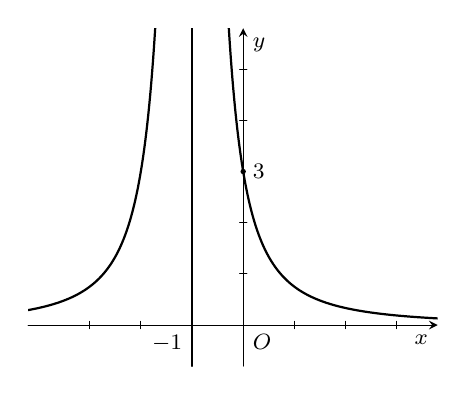
\begin{tikzpicture}[scale=0.65, font=\footnotesize, line join=round, line cap=round, >=stealth]
			\def\xmin{-4.2} \def\xmax{3.8}
			\def\ymin{-0.8} \def\ymax{5.8}
			\begin{scope}
				\clip (\xmin,\ymin) rectangle (\xmax,\ymax);
				\draw[thick] (-1,\ymin) -- (-1,\ymax);
				\draw[thick, samples=150, smooth, domain=\xmin:-1.7] plot (\x, {3/((\x)+1)^2});
				\draw[thick, samples=150, smooth, domain=-0.3:\xmax] plot (\x, {3/((\x)+1)^2});
			\end{scope}
			\draw[->] (\xmin,0) -- (\xmax,0) node[below left] {$x$};
			\draw[->] (0,\ymin) -- (0,\ymax) node[below right] {$y$};
			\foreach \x in {-3,-2,1,2,3} \draw (\x,2pt) -- (\x,-2pt);
			\foreach \y in {1,2,4,5} \draw (2pt,\y) -- (-2pt,\y);
			\node[below left] at (-1,0) {$-1$};
			\node[below right] at (0,0) {$O$};
			\node[right] at (0,3) {$3$};
			\fill (0,3) circle (1.5pt);
		\end{tikzpicture}
	}
	% [TỰ GIẢI - CẦN KIỂM TRA]
	\loigiai{
		\begin{itemchoice}
			\itemch Đúng. Từ đồ thị hàm số $y=f'(x)$, ta thấy trên khoảng $(-1;+\infty)$ đồ thị nằm phía trên trục hoành nên $f'(x)>0$, $\forall x\in(-1;+\infty)$.\\
			Do đó hàm số $y=f(x)$ đồng biến trên khoảng $(-1;+\infty)$.
			\itemch Sai. Vì hàm số $y=f(x)$ đồng biến trên đoạn $[0;2]\subset(-1;+\infty)$ nên
			\[ \max\limits_{[0;2]}f(x)=f(2)=1>f(0). \]
			\itemch Đúng. Đồ thị hàm số nhận $x=-1$ làm tiệm cận đứng nên $-\dfrac{d}{c}=-1\Leftrightarrow d=c\ne 0$.\\
			Chia cả tử và mẫu cho $c$, ta viết lại $f(x)=\dfrac{mx+n}{x+1}$, suy ra $f'(x)=\dfrac{m-n}{(x+1)^2}$.\\
			Đồ thị hàm số $y=f'(x)$ đi qua điểm $(0;3)$ nên $f'(0)=3\Leftrightarrow m-n=3\Leftrightarrow n=m-3$.\\
			Mặt khác $f(2)=1\Leftrightarrow\dfrac{2m+n}{3}=1\Leftrightarrow 2m+(m-3)=3\Leftrightarrow m=2\Rightarrow n=-1$.\\
			Suy ra $f(x)=\dfrac{2x-1}{x+1}$ có tiệm cận ngang là đường thẳng $y=2$.
			\itemch Sai. Ta có $f(x)=\dfrac{2x-1}{x+1}=2-\dfrac{3}{x+1}$.\\
			Với $x\in\mathbb{Z}$, để $f(x)\in\mathbb{Z}$ thì $(x+1)$ phải là ước nguyên của $3$, tức là $x+1\in\{-3;-1;1;3\}$.\\
			Vậy chỉ có $4$ điểm có tọa độ nguyên thuộc đồ thị hàm số $y=f(x)$.
		\end{itemchoice}
	}
\end{ex}

% Trang PDF: 2
\begin{ex}
	Cho hình chóp $S.ABCD$ có $SA\perp(ABCD)$ và đáy $ABCD$ là hình thoi tâm $O$, cạnh $AB=2$, $AC=2$, $SA=1$. Gọi $M$ là trung điểm của $SD$.
	\choiceTF
	{\True Diện tích hình thoi $ABCD$ bằng $2\sqrt{3}$}
	{\True Góc giữa hai đường thẳng $SO$ và $BD$ bằng $90^{\circ}$}
	{Diện tích tam giác $MAC$ bằng $\dfrac{3}{4}$}
	{Góc nhị diện $[M,AC,D]$ bằng $60^{\circ}$}
	% [TỰ GIẢI - CẦN KIỂM TRA]
	\loigiai{
		\immini{
			\begin{itemchoice}
				\itemch Đúng. Hình thoi $ABCD$ có $AB=BC=CD=DA=AC=2$ nên $\triangle ABC$ và $\triangle ACD$ là hai tam giác đều cạnh $2$.\\
				Do đó $S_{ABCD}=2\cdot S_{\triangle ABC}=2\cdot\dfrac{2^2\sqrt{3}}{4}=2\sqrt{3}$.
				\itemch Đúng. Ta có $\heva{&BD\perp AC\text{ (tính chất hình thoi)}\\ &BD\perp SA\text{ (do }SA\perp(ABCD)\text{)}}\Rightarrow BD\perp(SAC)$.\\
				Vì $SO\subset(SAC)$ nên $BD\perp SO$, suy ra góc giữa $SO$ và $BD$ bằng $90^{\circ}$.
				\itemch Sai. Gọi $H$ là trung điểm của $AD$, khi đó $MH$ là đường trung bình của $\triangle SAD$ nên $MH\parallel SA$, $MH=\dfrac{1}{2}SA=\dfrac{1}{2}$ và $MH\perp(ABCD)$.\\
				Trong $(ABCD)$, kẻ $HK\perp AC$ tại $K$. Vì $\triangle ACD$ đều cạnh $2$ và $AH=1$ nên $HK=AH\sin 60^{\circ}=\dfrac{\sqrt{3}}{2}$.\\
				Do $AC\perp HK$ và $AC\perp MH$ nên $AC\perp MK$. Độ dài đường cao $MK$ của $\triangle MAC$ là
				\[ MK=\sqrt{MH^2+HK^2}=\sqrt{\left(\dfrac{1}{2}\right)^2+\left(\dfrac{\sqrt{3}}{2}\right)^2}=1. \]
				Diện tích tam giác $MAC$ là $S_{\triangle MAC}=\dfrac{1}{2}AC\cdot MK=\dfrac{1}{2}\cdot 2\cdot 1=1$.
				\itemch Sai. Ta có $\heva{&AC\perp HK\\ &AC\perp MK}$ nên góc phẳng nhị diện của góc nhị diện $[M,AC,D]$ là $\widehat{MKH}$.\\
				Xét $\triangle MHK$ vuông tại $H$, ta có $\tan\widehat{MKH}=\dfrac{MH}{HK}=\dfrac{1}{\sqrt{3}}\Rightarrow\widehat{MKH}=30^{\circ}$.
			\end{itemchoice}
		}{
			\begin{tikzpicture}[scale=0.85, font=\footnotesize, line join=round, line cap=round]
				\coordinate (A) at (0,0);
				\coordinate (B) at (-1.4,-1.3);
				\coordinate (D) at (3.2,0);
				\coordinate (C) at ($(B)+(D)-(A)$);
				\coordinate (S) at (0,2.6);
				\coordinate (O) at ($(A)!0.5!(C)$);
				\coordinate (M) at ($(S)!0.5!(D)$);
				\coordinate (H) at ($(A)!0.5!(D)$);
				\coordinate (K) at ($(A)!0.25!(C)$);
				\draw[dashed, thin] (S)--(A) (A)--(B) (A)--(D) (A)--(C) (B)--(D) (S)--(O) (M)--(H) (H)--(K) (M)--(K) (M)--(A);
				\draw[thick] (S)--(B) (S)--(C) (S)--(D) (B)--(C) (C)--(D) (M)--(C);
				\foreach \p/\pos in {S/above, A/above left, B/below left, C/below right, D/right, O/below, M/above right, H/above, K/below left}
				\fill (\p) circle (1.2pt) node[\pos] {$\p$};
			\end{tikzpicture}
		}
	}
\end{ex}

% Trang PDF: 3
\begin{ex}
	Một con rô bốt hút bụi thông minh tự động di chuyển giữa $3$ vị trí được đánh số $A$, $B$, $C$ trong một phòng trưng bày, nếu đang ở vị trí này thì sau đúng $1$ phút, nó sẽ ở vị trí khác, theo quy tắc xác suất sau:
	\begin{itemize}
		\item Nếu đang ở vị trí $A$, rô bốt sẽ sang vị trí $B$ hoặc vị trí $C$ với xác suất đều bằng $0{,}5$.
		\item Nếu đang ở vị trí $B$, xác suất sang vị trí $A$ là $0{,}6$ và sang vị trí $C$ là $0{,}4$.
		\item Nếu đang ở vị trí $C$, xác suất sang vị trí $A$ là $0{,}8$ và sang vị trí $B$ là $0{,}2$.
	\end{itemize}
	Ban đầu, tại thời điểm ban đầu $t=0$ (phút), rô bốt đang ở vị trí $A$.
	\choiceTF
	{\True Xác suất để rô bốt ở vị trí $A$ tại thời điểm $t=1$ (phút) là $p_1=0$}
	{\True Xác suất để rô bốt ở vị trí $A$ tại thời điểm $t=2$ (phút) là $p_2=0{,}7$}
	{Tại thời điểm $t=3$ (phút), trong các vị trí $A$, $B$, $C$ thì xác suất rô bốt ở vị trí $A$ là lớn nhất}
	{\True Xác suất để rô bốt trở lại vị trí $A$ lần đầu tiên tại thời điểm $t=5$ (phút) là $p_5=0{,}0176$}
	% [TỰ GIẢI - CẦN KIỂM TRA]
	\loigiai{
		Gọi $a_n$, $b_n$, $c_n$ lần lượt là xác suất rô bốt ở vị trí $A$, $B$, $C$ tại thời điểm $t=n$ (phút). Ta có $(a_0;b_0;c_0)=(1;0;0)$.
		\begin{itemchoice}
			\itemch Đúng. Tại thời điểm $t=1$, rô bốt từ $A$ bắt buộc sang $B$ hoặc $C$ nên $p_1=a_1=0$, $b_1=0{,}5$, $c_1=0{,}5$.
			\itemch Đúng. Tại thời điểm $t=2$, xác suất rô bốt ở vị trí $A$ là
			\[ p_2=a_2=0{,}6b_1+0{,}8c_1=0{,}6\cdot 0{,}5+0{,}8\cdot 0{,}5=0{,}7. \]
			\itemch Sai. Tại thời điểm $t=2$, ta có $b_2=0{,}2c_1=0{,}1$ và $c_2=0{,}4b_1=0{,}2$.\\
			Suy ra tại thời điểm $t=3$:
			\[ \heva{&a_3=0{,}6b_2+0{,}8c_2=0{,}6\cdot 0{,}1+0{,}8\cdot 0{,}2=0{,}22\\ &b_3=0{,}5a_2+0{,}2c_2=0{,}5\cdot 0{,}7+0{,}2\cdot 0{,}2=0{,}39\\ &c_3=0{,}5a_2+0{,}4b_2=0{,}5\cdot 0{,}7+0{,}4\cdot 0{,}1=0{,}39.} \]
			Do đó tại $t=3$, xác suất rô bốt ở vị trí $A$ là nhỏ nhất ($0{,}22<0{,}39$).
			\itemch Đúng. Để rô bốt trở lại vị trí $A$ lần đầu tiên tại thời điểm $t=5$, trong các thời điểm $t=1,2,3,4$ rô bốt chỉ di chuyển luân phiên giữa $B$ và $C$ theo một trong hai lộ trình: $A\to B\to C\to B\to C\to A$ hoặc $A\to C\to B\to C\to B\to A$.\\
			Xác suất cần tìm là
			\[ p_5=0{,}5\cdot 0{,}4\cdot 0{,}2\cdot 0{,}4\cdot 0{,}8+0{,}5\cdot 0{,}2\cdot 0{,}4\cdot 0{,}2\cdot 0{,}6=0{,}0128+0{,}0048=0{,}0176. \]
		\end{itemchoice}
	}
\end{ex}
\Closesolutionfile{ans}

\Opensolutionfile{ans}[ans/ans-3]
\subsection*{Phần III. (3,0 điểm).} Thí sinh trả lời từ câu 1 đến câu 6.
\setcounter{ex}{0}

\begin{ex}
	Một nhóm gồm $9$ bạn học sinh, trong đó có Trí và Lan. Các bạn cùng chơi trò chơi tàu lượn siêu tốc gồm $3$ toa nối tiếp nhau: Toa 1, Toa 2 và Toa 3. Biết mỗi toa phải có ít nhất $1$ người, gọi $p$ là xác suất để Toa 1 chỉ có đúng $2$ người là Trí và Lan, tính giá trị $42p$.
	\shortans[0]{0,25}
	\loigiai{
		Ta xem thứ tự ngồi của các bạn trong mỗi toa là có phân biệt (mỗi cách xếp chỗ là một kết quả đồng khả năng).\\
		Xếp $9$ bạn học sinh thành một hàng dọc có $9!$ cách, sau đó đặt $2$ vách ngăn vào $8$ khoảng trống giữa $9$ bạn để chia thành $3$ toa nối tiếp nhau (mỗi toa có ít nhất $1$ người) có $\mathrm{C}_8^2=28$ cách.\\
		Số phần tử của không gian mẫu là $n(\Omega)=9!\cdot\mathrm{C}_8^2$.\\
		Để Toa 1 chỉ có đúng $2$ người là Trí và Lan: xếp Trí và Lan vào $2$ vị trí đầu hàng có $2!$ cách, xếp $7$ bạn còn lại vào $7$ vị trí sau có $7!$ cách, đặt vách ngăn thứ nhất ngay sau vị trí thứ hai có $1$ cách, đặt vách ngăn thứ hai vào $6$ khoảng trống giữa $7$ bạn còn lại có $\mathrm{C}_6^1=6$ cách.\\
		Suy ra xác suất cần tìm là
		\[ p=\dfrac{2!\cdot 7!\cdot 6}{9!\cdot\mathrm{C}_8^2}=\dfrac{12}{72\cdot 28}=\dfrac{1}{168}. \]
		Khi đó $42p=42\cdot\dfrac{1}{168}=0{,}25$.\\
		Vậy $42p=0{,}25$.
	}
\end{ex}

% Trang PDF: 3
\begin{ex}
	Trong một hệ thống trí tuệ nhân tạo (AI) dùng camera để nhận diện vật thể, camera được gắn trên một mô-tơ có thể quay liên tục. Khi camera quay quanh vật thể, góc nhìn thay đổi, làm cho chất lượng các đặc trưng hình ảnh mà hệ thống thu nhận cũng thay đổi.\\
	Hệ thống sử dụng hai thuật toán nhận diện độc lập. Với mỗi góc quay $x$ (đơn vị radian), $0\le x\le 8\pi$, mỗi thuật toán đưa ra một chỉ số tin cậy cho kết quả nhận diện. Qua quá trình thử nghiệm, các kỹ sư mô hình hóa hai chỉ số tin cậy này lần lượt bởi các hàm số $f(x)=1+\sin^2 x$ và $g(x)=1+\cos^2 x$.\\
	Để đánh giá mức độ phối hợp của hai thuật toán, hệ thống sử dụng một chỉ số kết hợp là $H(x)=\log_4 f(x)\cdot\log_4 g(x)$.\\
	Gọi $H_0=\log_4\dfrac{3}{2}$ và hệ thống đạt trạng thái phối hợp tối ưu khi $\sqrt{H(x)}=H_0$.\\
	Gọi $S$ là tổng tất cả các góc quay $x\in[0;8\pi]$ tại đó hệ thống đạt trạng thái phối hợp tối ưu, tính $\dfrac{20S}{\pi}$.
	\shortans[0]{$1280$}
	% [TỰ GIẢI - CẦN KIỂM TRA]
	\loigiai{
		Ta có $\log_4\left(1+\sin^2 x\right)\ge 0$ và $\log_4\left(1+\cos^2 x\right)\ge 0$, $\forall x\in[0;8\pi]$.\\
		Áp dụng bất đẳng thức AM-GM, ta có
		\[ \sqrt{H(x)}\le\dfrac{\log_4\left(1+\sin^2 x\right)+\log_4\left(1+\cos^2 x\right)}{2}=\dfrac{1}{2}\log_4\left[\left(1+\sin^2 x\right)\left(1+\cos^2 x\right)\right]. \]
		Mặt khác $\left(1+\sin^2 x\right)\left(1+\cos^2 x\right)=2+\sin^2 x\cos^2 x=2+\dfrac{1}{4}\sin^2 2x\le\dfrac{9}{4}$.\\
		Suy ra $\sqrt{H(x)}\le\dfrac{1}{2}\log_4\dfrac{9}{4}=\log_4\dfrac{3}{2}=H_0$.\\
		Đẳng thức $\sqrt{H(x)}=H_0$ xảy ra khi và chỉ khi $\sin^2 x=\cos^2 x=\dfrac{1}{2}\Leftrightarrow\cos 2x=0\Leftrightarrow x=\dfrac{\pi}{4}+k\dfrac{\pi}{2}$ $(k\in\mathbb{Z})$.\\
		Do $x\in[0;8\pi]$ nên $0\le\dfrac{\pi}{4}+k\dfrac{\pi}{2}\le 8\pi\Leftrightarrow k\in\{0;1;2;\dots;15\}$ (có $16$ giá trị).\\
		Tổng tất cả các góc quay thỏa mãn là $S=\dfrac{16}{2}\left(\dfrac{\pi}{4}+\dfrac{31\pi}{4}\right)=64\pi$.\\
		Suy ra $\dfrac{20S}{\pi}=\dfrac{20\cdot 64\pi}{\pi}=1280$.\\
		Vậy kết quả cần tìm là $1280$.
	}
\end{ex}

% Trang PDF: 3
\begin{ex}
	Một số có $12$ chữ số được gọi là số thú vị nếu các chữ số của nó bé hơn $9$ và khi tăng mỗi chữ số lên tối đa một đơn vị (mỗi chữ số có thể không tăng hoặc tăng thêm một đơn vị) thì ta được một số mới khác số ban đầu và chia hết cho số ban đầu. Hỏi có bao nhiêu số thú vị?
	\shortans[0]{$2048$}
	% [TỰ GIẢI - CẦN KIỂM TRA]
	\loigiai{
		Gọi $N=\overline{a_1a_2\dots a_{12}}$ là một số thú vị có $12$ chữ số ($a_1\ge 1$; $a_i\le 8$, $\forall i=1,\dots,12$).\\
		Khi tăng mỗi chữ số của $N$ lên tối đa $1$ đơn vị, ta được số mới là $M=N+D$, trong đó $D=\overline{d_1d_2\dots d_{12}}>0$ có các chữ số $d_i\in\{0;1\}$.\\
		Vì $M>N$ và $M\vdots N$ nên $M=kN$ với $k\in\mathbb{N}$, $k\ge 2$, suy ra $D=(k-1)N\ge N$.\\
		Mặt khác $N\ge 10^{11}$ và $D\le\underbrace{11\dots 1}_{12\text{ chữ số 1}}<2\cdot 10^{11}$ nên buộc phải có $k-1=1\Leftrightarrow D=N$.\\
		Do đó $N=D=\overline{d_1d_2\dots d_{12}}$ có chữ số đầu tiên $d_1=1$ và $11$ chữ số còn lại $d_2,d_3,\dots,d_{12}\in\{0;1\}$.\\
		Số các số thú vị là $1\cdot 2^{11}=2048$.\\
		Vậy có $2048$ số thú vị.
	}
\end{ex}

\begin{ex}
	Cho hình lăng trụ đứng $ABCD.A'B'C'D'$ có đáy $ABCD$ là hình thang cân, $AD$ song song $BC$, $AB=BC=CD=7\sqrt{6}$, $AD=14\sqrt{6}$. Góc giữa mặt phẳng $(A'CD)$ và $(ABCD)$ bằng $45^{\circ}$. Tính khoảng cách từ $B$ đến mặt phẳng $(A'CD)$.
	\shortans[0]{10,5}
	\loigiai{
		\immini{
			Đặt $a=7\sqrt{6}$. Khi đó hình thang cân $ABCD$ có $AB=BC=CD=a$ và đáy lớn $AD=2a$ là nửa lục giác đều nội tiếp đường tròn đường kính $AD$, suy ra $AC\perp CD$ và $AC=a\sqrt{3}$.\\
			Ta có $\heva{&CD\perp AC\\ &CD\perp AA'}\Rightarrow CD\perp(A'AC)\Rightarrow CD\perp A'C$.\\
			Do đó góc giữa hai mặt phẳng $(A'CD)$ và $(ABCD)$ là $\widehat{A'CA}=45^{\circ}$.\\
			Trong $\triangle A'AC$ vuông cân tại $A$, kẻ đường cao $AH\perp A'C$ tại $H$. Vì $CD\perp(A'AC)$ nên $CD\perp AH$, suy ra $AH\perp(A'CD)$.\\
			Ta có $\mathrm{d}\left(A,(A'CD)\right)=AH=\dfrac{AC}{\sqrt{2}}=\dfrac{7\sqrt{6}\cdot\sqrt{3}}{\sqrt{2}}=21$.\\
			Gọi $E$ là giao điểm của $AB$ và $CD$. Vì $BC\parallel AD$ và $BC=\dfrac{1}{2}AD$ nên $BC$ là đường trung bình của $\triangle EAD$, suy ra $B$ là trung điểm của $EA$.\\
			Vì $E\in CD\subset(A'CD)$ nên $\dfrac{\mathrm{d}\left(B,(A'CD)\right)}{\mathrm{d}\left(A,(A'CD)\right)}=\dfrac{EB}{EA}=\dfrac{1}{2}$.\\
			Suy ra $\mathrm{d}\left(B,(A'CD)\right)=\dfrac{21}{2}=10{,}5$.\\
			Vậy khoảng cách từ $B$ đến mặt phẳng $(A'CD)$ bằng $10{,}5$.
		}{
			\begin{tikzpicture}[scale=0.8, font=\footnotesize, line join=round, line cap=round]
				\coordinate (A) at (0,0);
				\coordinate (D) at (3.6,0);
				\coordinate (B) at (0.8,-1.2);
				\coordinate (C) at (2.8,-1.2);
				\coordinate (A') at (0,2.6);
				\coordinate (D') at (3.6,2.6);
				\coordinate (B') at (0.8,1.4);
				\coordinate (C') at (2.8,1.4);
				\coordinate (H) at ($(A')!0.5!(C)$);
				\draw[dashed, thin] (A)--(D) (A)--(C) (A')--(C) (A)--(H);
				\draw[thick] (A)--(B)--(C)--(D) (A')--(B')--(C')--(D')--(A') (A)--(A') (B)--(B') (C)--(C') (D)--(D') (A')--(D);
				\foreach \p/\pos in {A/left, B/below left, C/below right, D/right, A'/above left, B'/above left, C'/above, D'/above right, H/above right}
				\fill (\p) circle (1.2pt) node[\pos] {$\p$};
			\end{tikzpicture}
		}
	}
\end{ex}

% Trang PDF: 3
\begin{ex}
	Biết hàm số bậc ba $y=ax^3+bx^2+cx+d$ có bảng biến thiên như sau:
	\begin{center}
		
\begin{tikzpicture}
			\tkzTabInit[nocadre=false,lgt=1.2,espcl=2.5,deltacl=0.6]
			{$x$/0.6,$y'$/0.6,$y$/2}
			{$-\infty$,$-1$,$4$,$+\infty$}
			\tkzTabLine{,+,0,-,0,+,}
			\tkzTabVar{-/$-\infty$,+/$10$,-/$-22$,+/$+\infty$}
		\end{tikzpicture}
	\end{center}
	Biết rằng đồ thị hàm số trên cắt trục hoành tại ba điểm phân biệt có hoành độ lần lượt là $x_1$, $x_2$, $x_3$. Tính giá trị của $S=\dfrac{x_1+x_2+x_3}{2}$.
	\shortans[0]{$2{,}25$}
	% [TỰ GIẢI - CẦN KIỂM TRA]
	\loigiai{
		Từ bảng biến thiên, phương trình $y'=3ax^2+2bx+c=0$ có hai nghiệm phân biệt là $x=-1$ và $x=4$.\\
		Theo định lý Vi-ét đối với phương trình bậc hai $y'=0$, ta có
		\[ -\dfrac{2b}{3a}=(-1)+4=3\Rightarrow -\dfrac{b}{a}=\dfrac{9}{2}. \]
		Hoành độ giao điểm $x_1$, $x_2$, $x_3$ của đồ thị hàm số với trục hoành là ba nghiệm của phương trình $ax^3+bx^2+cx+d=0$.\\
		Theo định lý Vi-ét đối với phương trình bậc ba, ta có $x_1+x_2+x_3=-\dfrac{b}{a}=\dfrac{9}{2}$.\\
		Suy ra $S=\dfrac{x_1+x_2+x_3}{2}=\dfrac{9}{4}=2{,}25$.\\
		Vậy $S=2{,}25$.
	}
\end{ex}

% Trang PDF: 4
\begin{ex}
	\immini{
		Cho bảng vuông gồm $5\times 5$ ô vuông con, mỗi ô được điền một số sao cho trên mỗi hàng tính từ trái qua các số theo thứ tự là các số hạng liên tiếp của một cấp số cộng, các số trên mỗi cột tính từ trên xuống theo thứ tự cũng là các số hạng liên tiếp của một cấp số cộng. Do sơ suất nên trên bảng vuông chỉ còn xuất hiện một số số như hình vẽ bên. Gọi $x$ là số được điền vào ô của bảng như hình dưới, tính giá trị của $10x^2$.
		\shortans[0]{$1440$}
	}{
		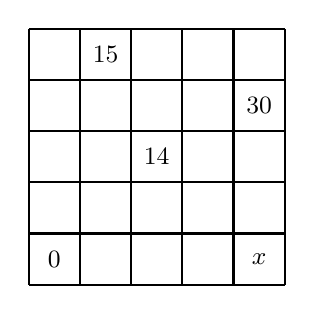
\begin{tikzpicture}[scale=0.65, font=\small]
			\draw[thick] (0,0) grid (5,5);
			\node at (1.5,4.5) {$15$};
			\node at (4.5,3.5) {$30$};
			\node at (2.5,2.5) {$14$};
			\node at (0.5,0.5) {$0$};
			\node at (4.5,0.5) {$x$};
		\end{tikzpicture}
	}
	% [TỰ GIẢI - CẦN KIỂM TRA]
	\loigiai{
		Gọi $a_{i,j}$ là số ở hàng thứ $i$ (tính từ trên xuống) và cột thứ $j$ (tính từ trái sang) với $i,j\in\{1;2;3;4;5\}$.\\
		Đặt $A=a_{1,1}$, $B=a_{1,5}$. Theo giả thiết ta có $a_{5,1}=0$ và $a_{5,5}=x$.\\
		Vì mỗi hàng và mỗi cột đều lập thành một cấp số cộng nên:
		\begin{itemize}
			\item Trên hàng $1$: $a_{1,2}=\dfrac{3A+B}{4}=15\Leftrightarrow 3A+B=60$.
			\item Trên cột $5$: $a_{2,5}=\dfrac{3B+x}{4}=30\Leftrightarrow 3B+x=120$.
			\item Ô chính giữa bảng $a_{3,3}$ là trung bình cộng của $4$ ô ở $4$ góc bảng:
			\[ a_{3,3}=\dfrac{a_{1,1}+a_{1,5}+a_{5,1}+a_{5,5}}{4}=14\Leftrightarrow A+B+x=56. \]
		\end{itemize}
		Giải hệ phương trình $\heva{&3A+B=60\\ &3B+x=120\\ &A+B+x=56}\Leftrightarrow\heva{&A=8\\ &B=36\\ &x=12.}$\\
		Khi đó $10x^2=10\cdot 12^2=1440$.\\
		Vậy $10x^2=1440$.
	}
\end{ex}
\Closesolutionfile{ans}

\Opensolutionfile{ans}[ans/ans-4]
\subsection*{Phần IV. Tự luận (10,0 điểm).} Thí sinh trả lời từ câu 1 đến câu 5.
\setcounter{ex}{0}

% Trang PDF: 4
\begin{ex}
	Sau $t$ tuần kể từ khi thả $5000$ con cá giống vào ao, khối lượng trung bình mỗi con cá được cho bởi công thức
	\[ w(t)=\dfrac{4+t-0{,}02t^2}{100}\text{ (kg)},\quad (0\le t\le 15). \]
	Do tỉ lệ hao hụt tự nhiên, số lượng cá còn sống trong ao sau $t$ tuần là
	\[ P(t)=\dfrac{5000}{t+10}\text{ (con)},\quad (0\le t\le 15). \]
	Sản lượng cá $y(t)$ thu được sau $t$ tuần là tổng khối lượng cá còn sống trong ao. Hỏi sau bao nhiêu tuần thì sản lượng cá thu hoạch được đạt giá trị lớn nhất?
	% [TỰ GIẢI - CẦN KIỂM TRA]
	\loigiai{
		Sản lượng cá $y(t)$ thu được sau $t$ tuần $(0\le t\le 15)$ là
		\[ y(t)=w(t)\cdot P(t)=\dfrac{4+t-0{,}02t^2}{100}\cdot\dfrac{5000}{t+10}=\dfrac{-t^2+50t+200}{t+10}\text{ (kg)}. \]
		Ta có đạo hàm của hàm số $y(t)$ trên đoạn $[0;15]$ là
		\[ y'(t)=\dfrac{(-2t+50)(t+10)-\left(-t^2+50t+200\right)}{(t+10)^2}=\dfrac{-t^2-20t+300}{(t+10)^2}. \]
		Cho $y'(t)=0\Leftrightarrow -t^2-20t+300=0\Leftrightarrow\hoac{&t=10\in[0;15]\\ &t=-30\notin[0;15].}$\\
		Bảng biến thiên của hàm số $y(t)$ trên đoạn $[0;15]$:
		\begin{center}
			
\begin{tikzpicture}
				\tkzTabInit[nocadre=false,lgt=1.2,espcl=2.5,deltacl=0.6]
				{$t$/0.6,$y'(t)$/0.6,$y(t)$/2}
				{$0$,$10$,$15$}
				\tkzTabLine{,+,0,-,}
				\tkzTabVar{-/$20$,+/$30$,-/$29$}
			\end{tikzpicture}
		\end{center}
		Từ bảng biến thiên, ta có $\max\limits_{[0;15]}y(t)=y(10)=30\text{ (kg)}$.\\
		Vậy sau $10$ tuần thì sản lượng cá thu hoạch được đạt giá trị lớn nhất (bằng $30\,$kg).
	}
\end{ex}

% Trang PDF: 4
\begin{ex}
	\begin{enumerate}[a)]
		\item Trong mặt phẳng tọa độ $Oxy$, gọi $A$, $B$ là hai điểm phân biệt thuộc đồ thị của hàm số $y=1+\log_3(x-1)$ sao cho $A$ là trung điểm $OB$. Tính độ dài đoạn thẳng $AB$.
		\item Tìm các số thực dương $a$, $b$, $c$ sao cho $a\ne 1$ và thỏa mãn đồng thời các đẳng thức sau:
		\[ b+\log_2 a=0,\quad \log_a b=\dfrac{1}{c},\quad \log_2\left(\dfrac{b}{c}\right)=c-b. \]
	\end{enumerate}
	% [TỰ GIẢI - CẦN KIỂM TRA]
	\loigiai{
		\begin{enumerate}[a)]
			\item Điều kiện xác định của hàm số là $x>1$.\\
			Gọi $A\left(x_A;1+\log_3(x_A-1)\right)$ với $x_A>1$.\\
			Vì $A$ là trung điểm của $OB$ nên tọa độ điểm $B$ là $B\left(2x_A;2+2\log_3(x_A-1)\right)$.\\
			Do điểm $B$ thuộc đồ thị hàm số $y=1+\log_3(x-1)$ nên ta có
			\[ 2+2\log_3(x_A-1)=1+\log_3(2x_A-1)\Leftrightarrow\log_3\left[3(x_A-1)^2\right]=\log_3(2x_A-1) \]
			\[ \Leftrightarrow 3(x_A-1)^2=2x_A-1\Leftrightarrow 3x_A^2-8x_A+4=0\Leftrightarrow\hoac{&x_A=2\text{ (thỏa mãn)}\\ &x_A=\dfrac{2}{3}\text{ (loại do }x_A>1\text{)}.} \]
			Suy ra $A(2;1)$ và $B(4;2)$.\\
			Vậy độ dài đoạn thẳng $AB$ là $AB=\sqrt{(4-2)^2+(2-1)^2}=\sqrt{5}$.
			\item Từ đẳng thức $\log_2\left(\dfrac{b}{c}\right)=c-b$, ta có $\log_2 b+b=\log_2 c+c$.\\
			Xét hàm số $f(t)=\log_2 t+t$ trên khoảng $(0;+\infty)$, ta có $f'(t)=\dfrac{1}{t\ln 2}+1>0$, $\forall t>0$ nên hàm số $f(t)$ đồng biến trên $(0;+\infty)$.\\
			Do đó $f(b)=f(c)\Leftrightarrow b=c$.\\
			Từ đẳng thức $b+\log_2 a=0$, ta có $\log_2 a=-b\Leftrightarrow a=2^{-b}$.\\
			Thay $a=2^{-b}$ và $c=b$ vào đẳng thức $\log_a b=\dfrac{1}{c}$, ta được
			\[ \log_{2^{-b}}b=\dfrac{1}{b}\Leftrightarrow -\dfrac{1}{b}\log_2 b=\dfrac{1}{b}\Leftrightarrow\log_2 b=-1\Leftrightarrow b=\dfrac{1}{2}. \]
			Suy ra $c=b=\dfrac{1}{2}$ và $a=2^{-\frac{1}{2}}=\dfrac{\sqrt{2}}{2}$ (thỏa mãn điều kiện $a,b,c>0$ và $a\ne 1$).\\
			Vậy $(a;b;c)=\left(\dfrac{\sqrt{2}}{2};\dfrac{1}{2};\dfrac{1}{2}\right)$.
		\end{enumerate}
	}
\end{ex}

% Trang PDF: 4
\begin{ex}
	Gọi $A$ là tập hợp tất cả các số tự nhiên có $5$ chữ số. Chọn ngẫu nhiên một số từ tập $A$, tính xác suất để chọn được một số chia hết cho $17$ và có chữ số hàng đơn vị bằng $3$.
	% [TỰ GIẢI - CẦN KIỂM TRA]
	\loigiai{
		Tập hợp $A=\{10000;10001;\dots;99999\}$ có $99999-10000+1=90000$ phần tử, nên $n(\Omega)=90000$.\\
		Gọi $n\in A$ là số tự nhiên có $5$ chữ số chia hết cho $17$ và có chữ số hàng đơn vị bằng $3$.\\
		Vì $n=17k$ $(k\in\mathbb{N})$ có chữ số tận cùng bằng $3$ nên $k$ phải có chữ số tận cùng bằng $9$, tức là $k=10m+9$ $(m\in\mathbb{N})$.\\
		Khi đó $n=17(10m+9)=170m+153$.\\
		Do $10000\le n\le 99999$ nên
		\[ 10000\le 170m+153\le 99999\Leftrightarrow\dfrac{9847}{170}\le m\le\dfrac{99846}{170}\Leftrightarrow 57{,}92\dots\le m\le 587{,}32\dots \]
		Vì $m\in\mathbb{N}$ nên $m\in\{58;59;\dots;587\}$, có $587-58+1=530$ giá trị của $m$, tương ứng với $530$ số thỏa mãn.\\
		Xác suất cần tìm là $P=\dfrac{530}{90000}=\dfrac{53}{9000}$.\\
		Vậy xác suất cần tìm là $\dfrac{53}{9000}$.
	}
\end{ex}

% Trang PDF: 4
\begin{ex}
	Cho hàm số $y=\dfrac{1}{x}$ có đồ thị là $(C_1)$ và hàm số $y=\dfrac{4}{x}$ có đồ thị là $(C_2)$.
	\begin{enumerate}[a)]
		\item Gọi $A$ là điểm thuộc đồ thị $(C_1)$ có hoành độ bằng $1$. Xác định tọa độ điểm $B$ thuộc đồ thị hàm số $(C_2)$ sao cho $AB$ đạt giá trị nhỏ nhất.
		\item Lấy $M$ là điểm bất kỳ thuộc đồ thị $(C_1)$ có hoành độ là $a$ $(a>1)$, gọi $N$ thuộc đồ thị hàm số $(C_2)$ sao cho $MN$ đạt giá trị nhỏ nhất. Chứng minh rằng $MN<AB$.
	\end{enumerate}
	% [TỰ GIẢI - CẦN KIỂM TRA]
	\loigiai{
		\begin{enumerate}[a)]
			\item Vì $A\in(C_1)$ có hoành độ bằng $1$ nên $A(1;1)$.\\
			Gọi $B\left(x;\dfrac{4}{x}\right)\in(C_2)$ $(x\ne 0)$. Khi đó $AB^2=(x-1)^2+\left(\dfrac{4}{x}-1\right)^2$.\\
			Nếu $x<0$ thì $x-1<-1$ và $\dfrac{4}{x}-1<-1$, suy ra $AB^2>1+1=2$.\\
			Nếu $x>0$, đặt $t=x+\dfrac{4}{x}\ge 2\sqrt{x\cdot\dfrac{4}{x}}=4$ (theo bất đẳng thức AM-GM).\\
			Ta có $AB^2=\left(x^2+\dfrac{16}{x^2}\right)-2\left(x+\dfrac{4}{x}\right)+2=t^2-2t-6=(t-1)^2-7\ge(4-1)^2-7=2$.\\
			Dấu bằng xảy ra khi và chỉ khi $t=4\Leftrightarrow x=\dfrac{4}{x}$ $(x>0)\Leftrightarrow x=2$.\\
			Vậy $AB$ đạt giá trị nhỏ nhất bằng $\sqrt{2}$ khi $B(2;2)$.
			\item Điểm $M\in(C_1)$ có hoành độ $a>1$ nên $M\left(a;\dfrac{1}{a}\right)$.\\
			Xét điểm $P\left(a+1;\dfrac{4}{a+1}\right)\in(C_2)$. Theo định nghĩa của điểm $N$, ta có $MN\le MP$.\\
			Ta tính khoảng cách $MP$:
			\[ MP^2=\left[(a+1)-a\right]^2+\left(\dfrac{4}{a+1}-\dfrac{1}{a}\right)^2=1+\left(\dfrac{3a-1}{a(a+1)}\right)^2. \]
			Với $a>1$, ta có $3a-1>2>0$ và $a(a+1)-(3a-1)=a^2-2a+1=(a-1)^2>0$.\\
			Suy ra $0<3a-1<a(a+1)\Rightarrow 0<\dfrac{3a-1}{a(a+1)}<1\Rightarrow\left(\dfrac{3a-1}{a(a+1)}\right)^2<1$.\\
			Do đó $MN^2\le MP^2<1+1=2=AB^2$, suy ra $MN<AB$ (điều phải chứng minh).
		\end{enumerate}
	}
\end{ex}

% Trang PDF: 4
\begin{ex}
	Một khối gỗ đặc có dạng hình chóp $S.ABCD$ với đáy $ABCD$ là hình chữ nhật, mặt bên $SAB$ là tam giác vuông cân có cạnh huyền bằng $2a$ và nằm trong mặt phẳng vuông góc với mặt đáy, đồng thời tam giác $SCD$ là tam giác đều.
	\begin{enumerate}[a)]
		\item Tính độ dài cạnh $AD$ theo $a$.
		\item Người ta muốn nối một sợi dây nằm trên bề mặt của khối gỗ từ trọng tâm tam giác $SAB$ đến trọng tâm tam giác $SCD$. Tính độ dài ngắn nhất của sợi dây theo $a$.
	\end{enumerate}
	% [TỰ GIẢI - CẦN KIỂM TRA]
	\loigiai{
		\begin{enumerate}[a)]
			\item
			\immini{
				Gọi $H$, $K$ lần lượt là trung điểm của $AB$ và $CD$.\\
				Vì $\triangle SAB$ vuông cân tại $S$ có cạnh huyền $AB=2a$ nên $SH\perp AB$ và $SH=\dfrac{1}{2}AB=a$.\\
				Do $(SAB)\perp(ABCD)$ theo giao tuyến $AB$ nên $SH\perp(ABCD)\Rightarrow SH\perp HK$.\\
				Tam giác $SCD$ đều cạnh $CD=AB=2a$ nên đường trung tuyến $SK=\dfrac{2a\sqrt{3}}{2}=a\sqrt{3}$.\\
				Xét $\triangle SHK$ vuông tại $H$, ta có $AD=HK=\sqrt{SK^2-SH^2}=\sqrt{3a^2-a^2}=a\sqrt{2}$.\\
				Vậy $AD=a\sqrt{2}$.
			}{
				\begin{tikzpicture}[scale=0.85, font=\footnotesize, line join=round, line cap=round]
					\coordinate (A) at (0,0);
					\coordinate (B) at (-1.4,-1.4);
					\coordinate (D) at (3.2,0);
					\coordinate (C) at ($(B)+(D)-(A)$);
					\coordinate (H) at ($(A)!0.5!(B)$);
					\coordinate (K) at ($(C)!0.5!(D)$);
					\coordinate (S) at ($(H)+(0,2.5)$);
					\coordinate (G1) at ($(S)!0.667!(H)$);
					\coordinate (G2) at ($(S)!0.667!(K)$);
					\draw[dashed, thin] (A)--(B) (A)--(D) (S)--(A) (S)--(H) (H)--(K);
					\draw[thick] (S)--(B) (S)--(C) (S)--(D) (B)--(C) (C)--(D) (S)--(K);
					\foreach \p/\pos in {S/above, A/above right, B/below left, C/below right, D/right, H/left, K/right, G1/left, G2/above right}
					\fill (\p) circle (1.2pt) node[\pos] {$\p$};
				\end{tikzpicture}
			}
			\item Gọi $G_1$, $G_2$ lần lượt là trọng tâm của $\triangle SAB$ và $\triangle SCD$. Ta có $SG_1=\dfrac{2}{3}SH=\dfrac{2a}{3}$ và $SG_2=\dfrac{2}{3}SK=\dfrac{2a\sqrt{3}}{3}$.\\
			Xét $\triangle SAD$ có $SA=a\sqrt{2}$, $AD=a\sqrt{2}$ và $SD=2a$. Vì $SA^2+AD^2=2a^2+2a^2=4a^2=SD^2$ nên $\triangle SAD$ vuông cân tại $A$, suy ra $\widehat{ASD}=45^{\circ}$.\\
			Mặt khác, trong $\triangle SAB$ vuông cân tại $S$ ta có $\widehat{G_1SA}=45^{\circ}$; trong $\triangle SCD$ đều ta có $\widehat{DSG_2}=30^{\circ}$.\\
			Trải phẳng ba mặt bên $(SAB)$, $(SAD)$, $(SCD)$ lên cùng một mặt phẳng xoay quanh các cạnh $SA$, $SD$, khi đó góc $\widehat{G_1SG_2}$ trên mặt phẳng trải là
			\[ \widehat{G_1SG_2}=\widehat{G_1SA}+\widehat{ASD}+\widehat{DSG_2}=45^{\circ}+45^{\circ}+30^{\circ}=120^{\circ}. \]
			Độ dài đường đi ngắn nhất từ $G_1$ đến $G_2$ qua các mặt bên là
			\[ L_1=G_1G_2=\sqrt{SG_1^2+SG_2^2-2\cdot SG_1\cdot SG_2\cdot\cos 120^{\circ}}=\sqrt{\dfrac{4a^2}{9}+\dfrac{12a^2}{9}+2\cdot\dfrac{2a}{3}\cdot\dfrac{2a\sqrt{3}}{3}\cdot\dfrac{1}{2}}=\dfrac{2a\sqrt{4+\sqrt{3}}}{3}. \]
			Nếu sợi dây đi qua mặt đáy $(ABCD)$ thì độ dài ngắn nhất là $L_2=G_1H+HK+KG_2=\dfrac{a}{3}+a\sqrt{2}+\dfrac{a\sqrt{3}}{3}>L_1$.\\
			Vậy độ dài ngắn nhất của sợi dây là $\dfrac{2a\sqrt{4+\sqrt{3}}}{3}$.
		\end{enumerate}
	}
\end{ex}
\Closesolutionfile{ans}

\dapan